\chapter{ADC Control 2 MS/s} \label{App:HSADCControlTest}
This appendix shows the considerations for the set sampling rate of the system.

The working principle for the sampling system was decided early on in the project, and the highest test frequency that has to be measured is \SIQ{1}{\mega\hertz} sine waves. The choice was between two principles, either the project samples at 2MS/s in order to adhere to the Nyquist sampling theorem, or a sub-sampling principle is used. Sub-sampling is where the anti-aliasing effect is exploited in order to sample the waveforms at lower sample rates. Ultimately it was decided to use the sub-sampling principle over concerns of signal fidelity on the physical PCB and uncertainties and memory data rates. The clock signals for the ADCs would have to be \textit{high} and high frequency square waves pose certain challenges that the project team doesn't have enough time to solve for this semester project. The digital system in the sample control module is designed to operate at higher sample rates than is actually used, so that the project can be switched to use the higher 2MS/s sample rates if the team wants to switch sampling principle, so this was also tested for the ADC control module.

The only change that the module requires in order to do this, is to change the SPI CLK frequency since all the other pulses, such as CVN, DCN and DSC as described in section \refq{fig:7_2_8_ADC_CONTROL_DCN_MEAS} are already designed for higher sample rates. The ADC control module uses the pulse generator from section \refq{subsec:PWMGen} to make the SPI CLK and simply changing the values of the 'HIGH' and 'LOW' period changes the SPI CLK frequency. This has been done in this 2 MS/s test.

On figure \refq{fig:A_HighSpeedADCControlTest_CNV} it can be seen that the distance between the CNV pulses, in yellow, is \SIQ{480}{\nano\second}. There is some error in this measurement due to manual cursor placement on the oscilloscope. This corresponds to a CNV frequency of \SIQ{2.083}{\mega\hertz} as shown on the right side of the screen.
\begin{figure}[H]
    \centering
    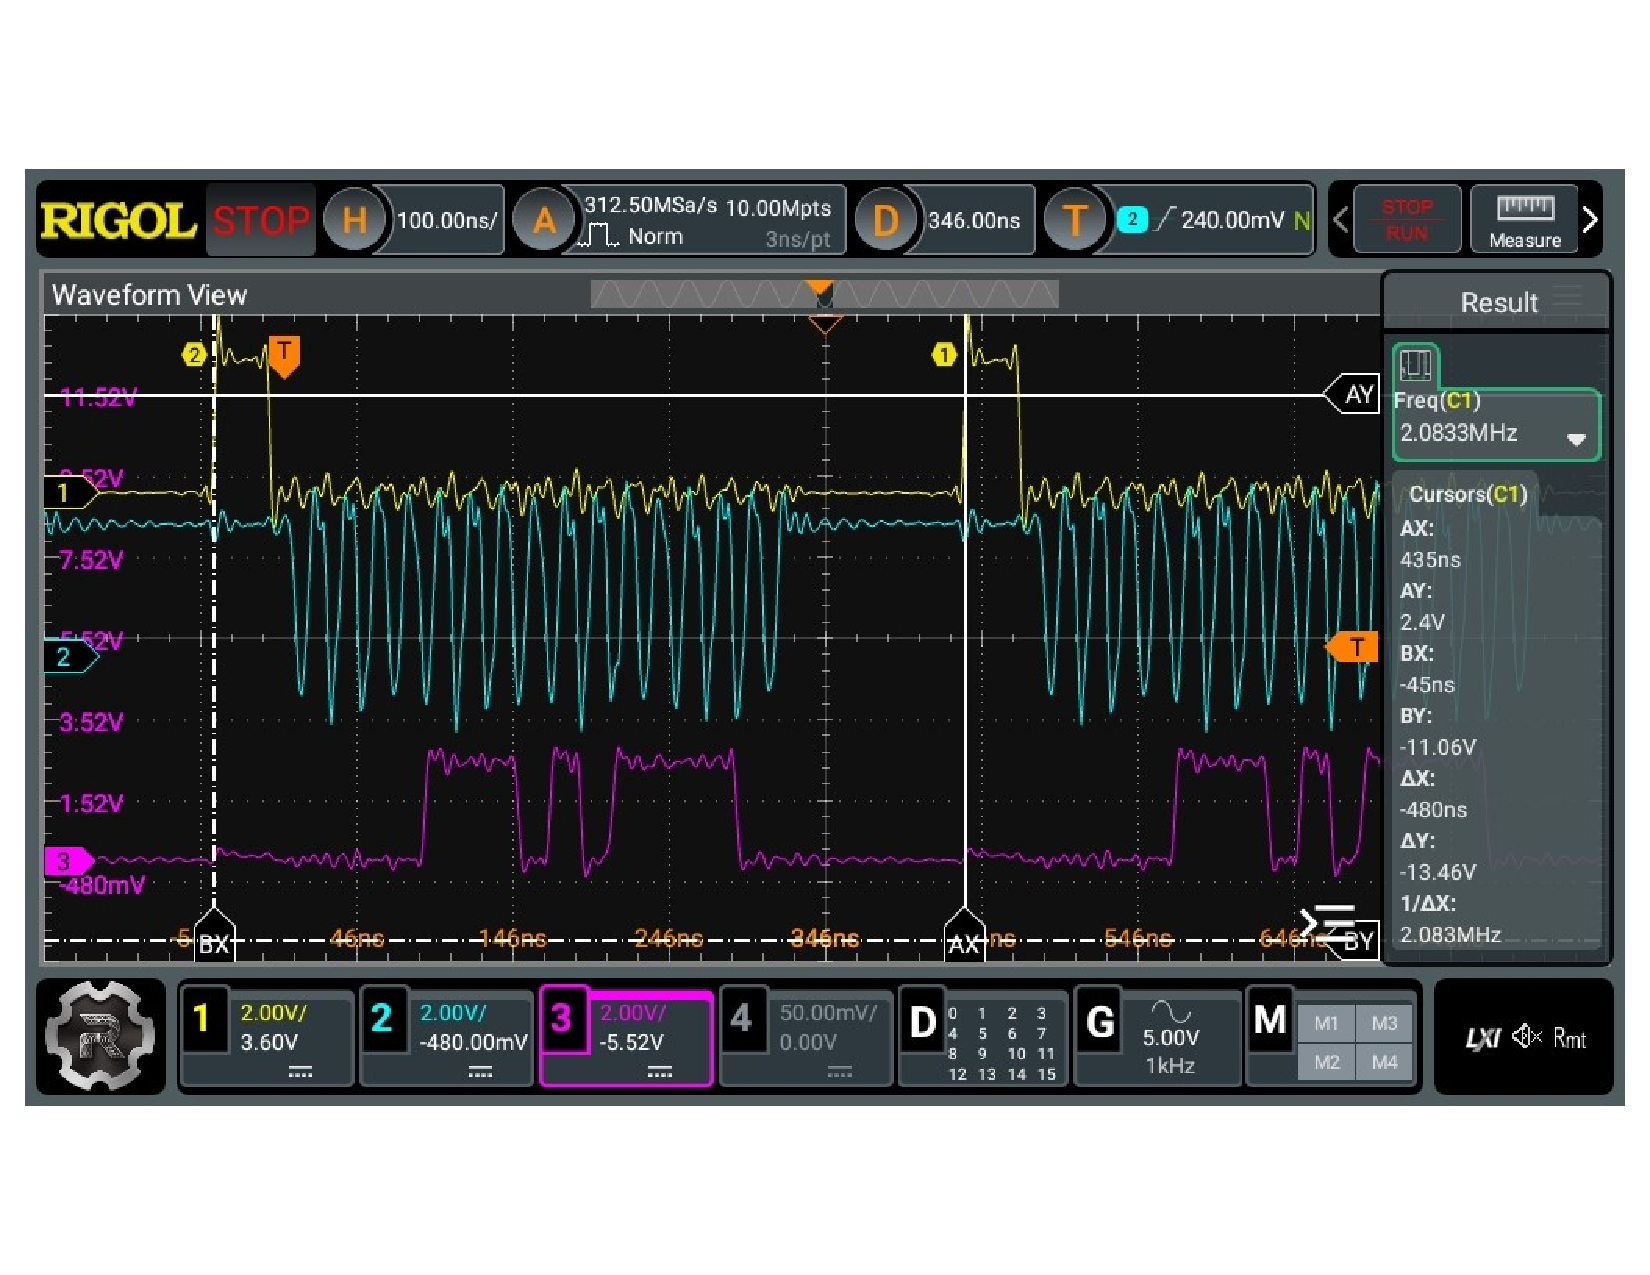
\includegraphics[clip, trim=0 75 0 50, width=0.9\textwidth]{Appendix/Figures/A_HighSpeedADCControlTestCNV.pdf}
    \caption{A measurement of the CNV frequency. The sample rate of the ADCs is equal to the CNV pulse frequency. Yellow is the CNV pulse, blue is the SPI CLK and red is the SPI data bus.}
    \label{fig:A_HighSpeedADCControlTest_CNV}
\end{figure}

The fidelity of the SPI CLK signal was of special interest so this was also measured on it's own. The results can be seen on figure \refq{fig:A_HighSpeedADCControlTest_SPICLK}

\begin{figure}[H]
    \centering
    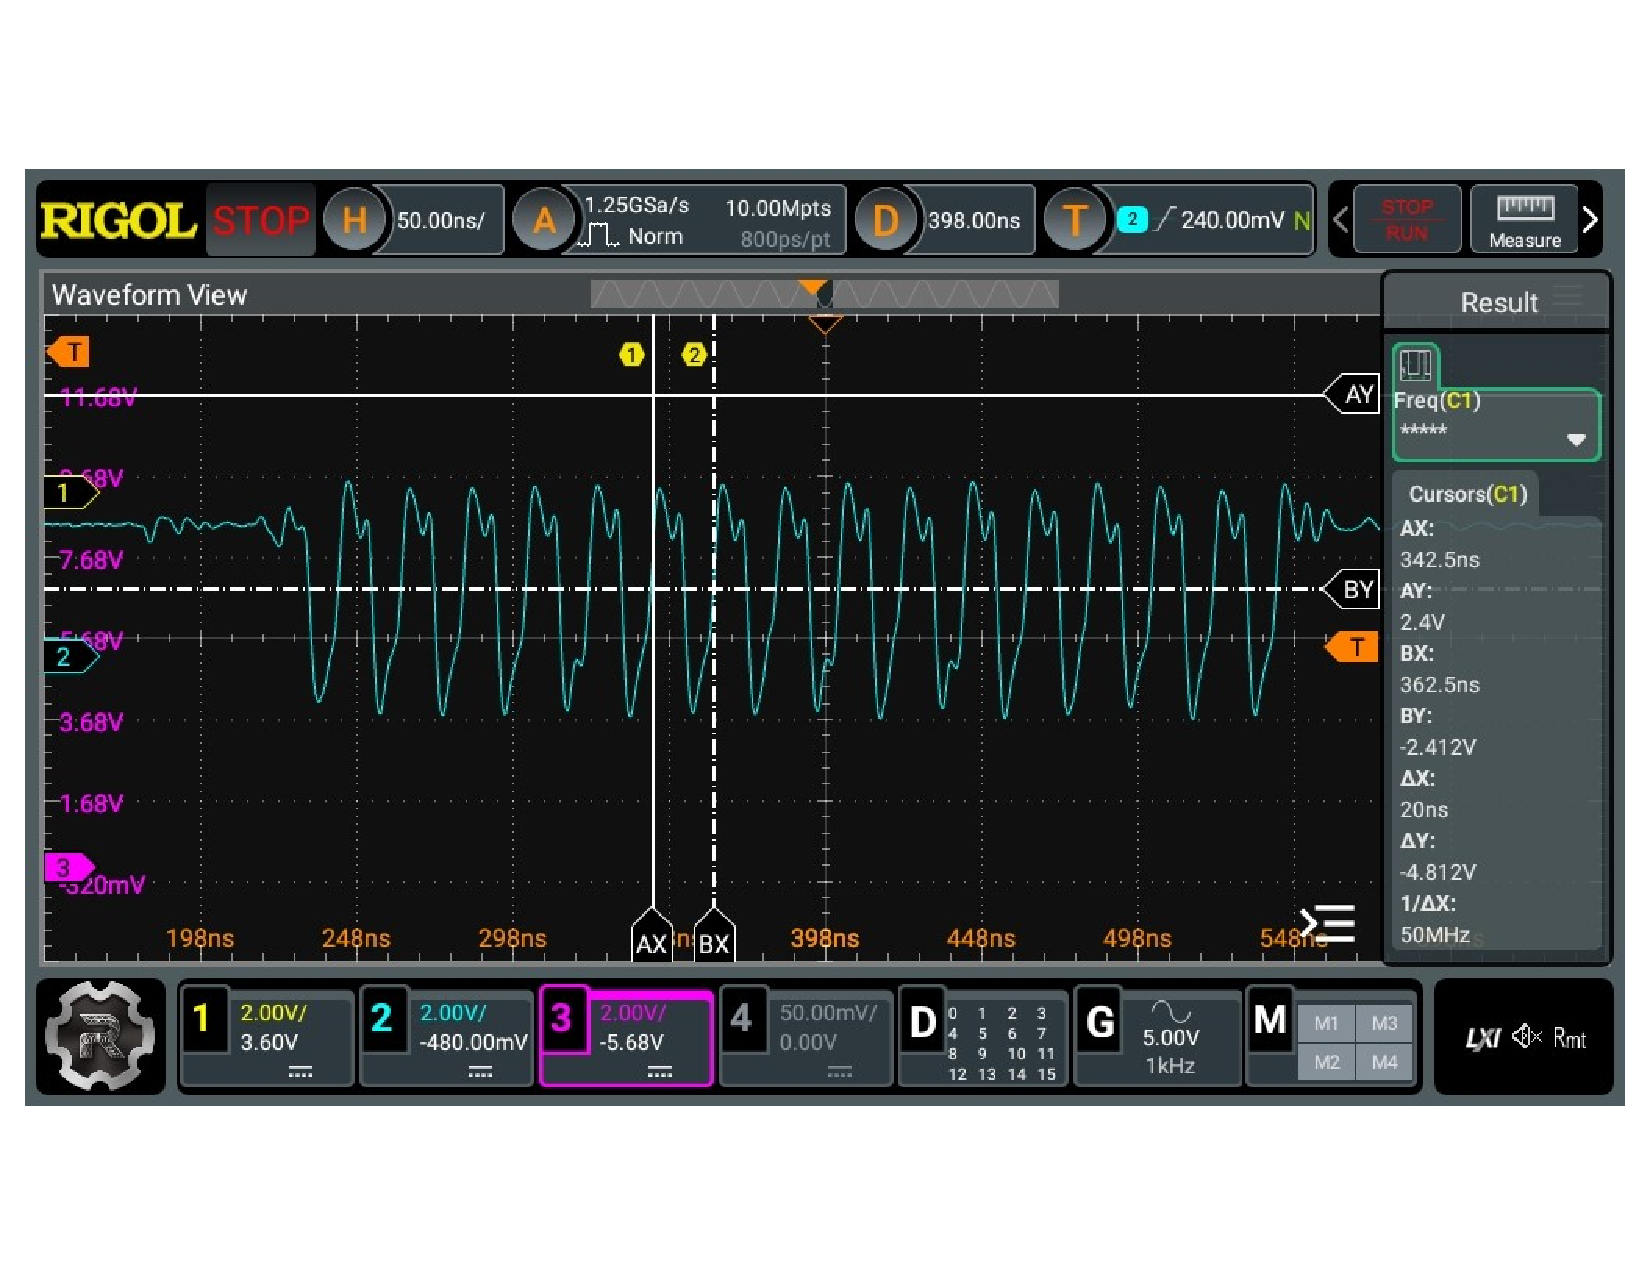
\includegraphics[clip, trim=0 75 0 50, width=0.9\textwidth]{Appendix/Figures/A_HighSpeedADCControlTestSPICLK.pdf}
    \caption{A measurement of the SPI CLK. With the modifications to the pulse generator that was described in this appendex, the SPI CLK frequency is 50MHz. Yellow is the CNV pulse, blue is the SPI CLK and red is the SPI data bus.}
    \label{fig:A_HighSpeedADCControlTest_SPICLK}
\end{figure}

The SPI CLK shown on figure \refq{fig:A_HighSpeedADCControlTest_SPICLK} is ,almost, more triangular shaped than it is a square wave, and quite noisy. There are various reasons for this. The oscilloscope input and probes are loading the SPI CLK bus, the SPI CLK is a single-ended signal and the FPGA may not be quite capable of driving the bus on it's own. Using the higher sample rate requires more time than is available for the project, to gain enough confidence in these high speed signals to implement it in practice, so the sub-sampling principle is used.